\section{Metodología}

Para la creación del filtro, se siguieron los pasos de la guía \textit{Advanced Design System-Circuit Design Cookbook 2.0. Keysight Technologies}~\cite{keysight_csc2}.

\subsection{Creación del layout}

Crear un nuevo layout haciendo click derecho sobre la carpeta del proyecto, seleccionar la opción \texttt{New layout}. \\

Abrir el archivo creado. Haciendo uso de la librería de \texttt{TLines-Microstrip}, utilizar el elemento \texttt{MLIN} para formar las secciones del filtro, esto se puede observar en la Figura \ref{fig:metologia_mlin}. 

\begin{figure}[h!]
    \centering
    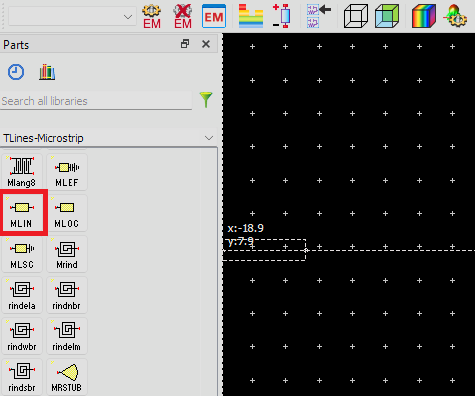
\includegraphics[width=8cm]{figures/metodologia/metologia1.png}
    \caption{Parte utilizada para dibujar las secciones del filtro}
    \label{fig:metologia_mlin}
\end{figure}

Colocar el elemento en el área de trabajo demarcado por la zona oscura. Una vez colocado el elemento, darle doble click izquierdo para abrir el panel de parámetros que se puede observar en la Figura \ref{fig:metologia_mlin_dimensiones}.

\begin{figure}[h!]
    \centering
    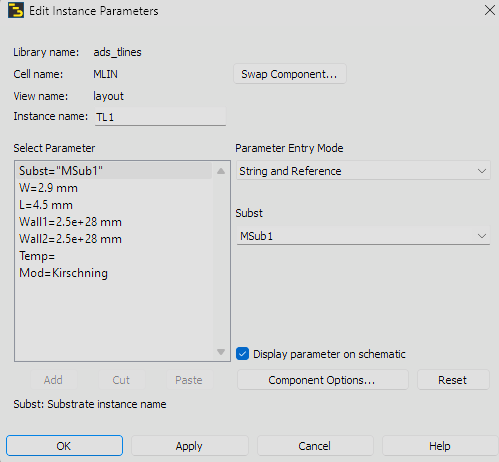
\includegraphics[width=8cm]{figures/metodologia/metologia2.png}
    \caption{Panel de parámetros del elemento \texttt{MLIN}}
    \label{fig:metologia_mlin_dimensiones}
\end{figure}

Con los pasos mencionados anteriormente, inserte las secciones necesarias utilizando los datos mostrados en la tabla \ref{table:metodologia_dimensiones} hasta formar la estructura mostrada en la figura \ref{fig:metologia_secciones_filtro}, donde el ancho corresponde al parámetro \texttt{W} y el largo a \texttt{L}.

\begin{table}[h!]
\centering
\caption{Dimensiones de las secciones del filtro}
\label{table:metodologia_dimensiones}
\begin{tabular}{|c|c|c|}
\hline
Sección & Ancho {[}mm{]} & Largo {[}mm{]} \\ \hline
TL1     & 2.9            & 4.5            \\ \hline
TL2     & 24.7           & 1.68           \\ \hline
TL3     & 0.66           & 10.145         \\ \hline
TL4     & 24.7           & 4.057          \\ \hline
TL5     & 0.66           & 4.202          \\ \hline
TL6     & 2.9            & 4.5            \\ \hline
\end{tabular}
\end{table}

\begin{figure}[h!]
    \centering
    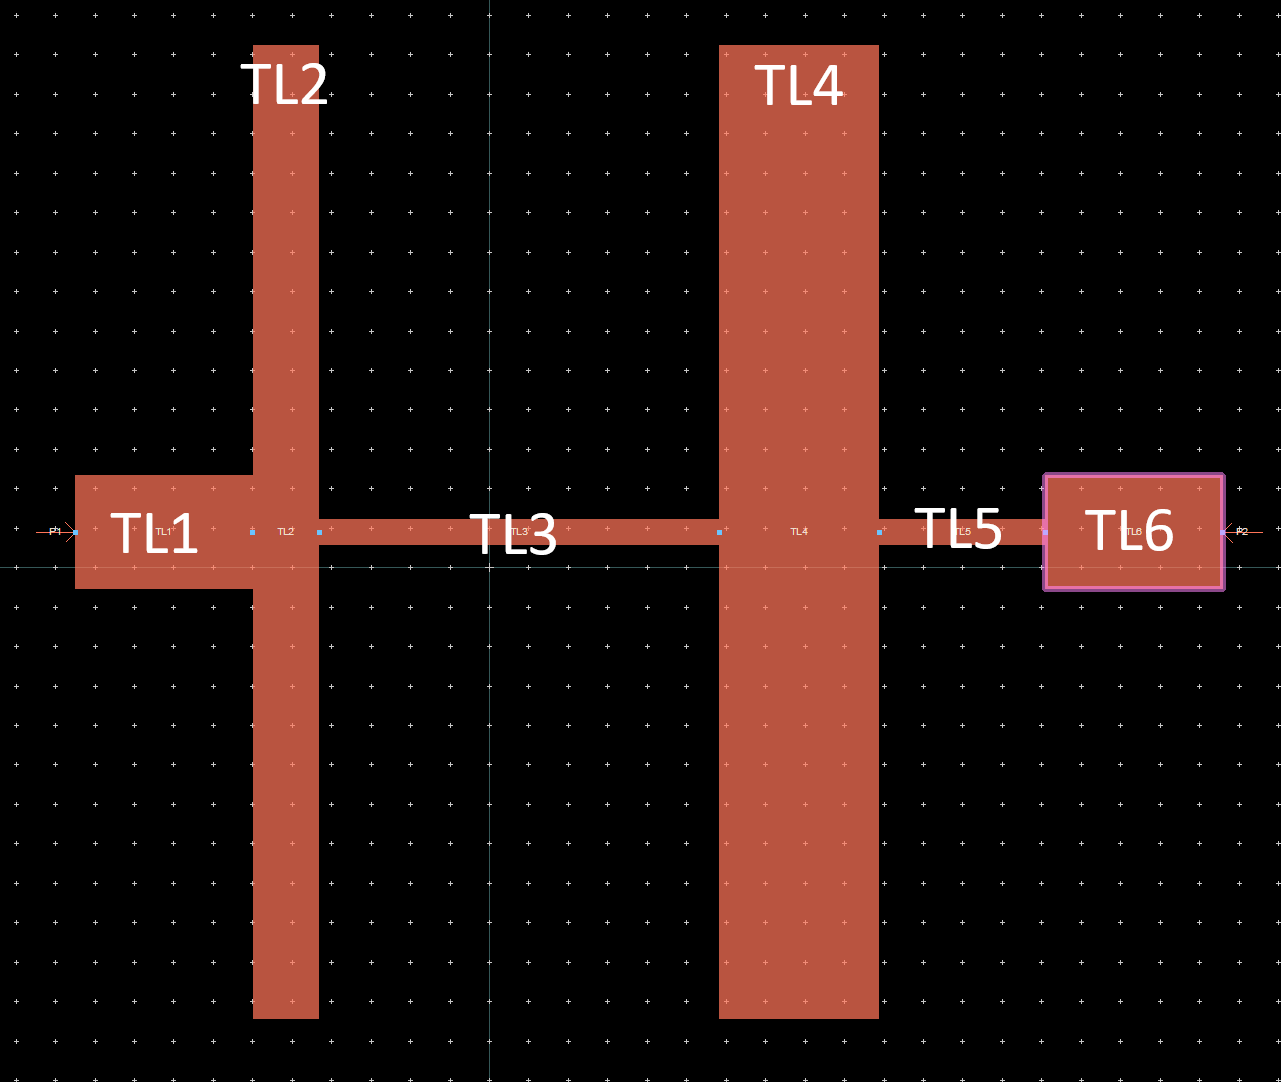
\includegraphics[width=8cm]{figures/metodologia/metologia3.png}
    \caption{Secciones del filtro}
    \label{fig:metologia_secciones_filtro}
\end{figure}

Una vez completada la estructura del filtro, puede proceder a agregar los pines para la simulación \texttt{EM}, para eso haga click en \texttt{Insert} y seleccione la opción \texttt{Pin}. Coloque uno en la conexión restante de \texttt{TL1} y otro en la conexión restante de \texttt{TL6}.

\subsection{Creación del substrato}

Crear un nuevo substrato haciendo click derecho sobre la carpeta del proyecto, seleccionar la opción \texttt{New substrate}. \\

Modifique el substrato para que se vea como el mostrado en la figura \ref{fig:metologia_substrato}. La capa del dieléctrico debe tener una constante de permeabilidad de 4.6, una tangente de pérdidas de $0.0023$, y un espesor de 1.6mm.
\begin{figure}[h!]
    \centering
    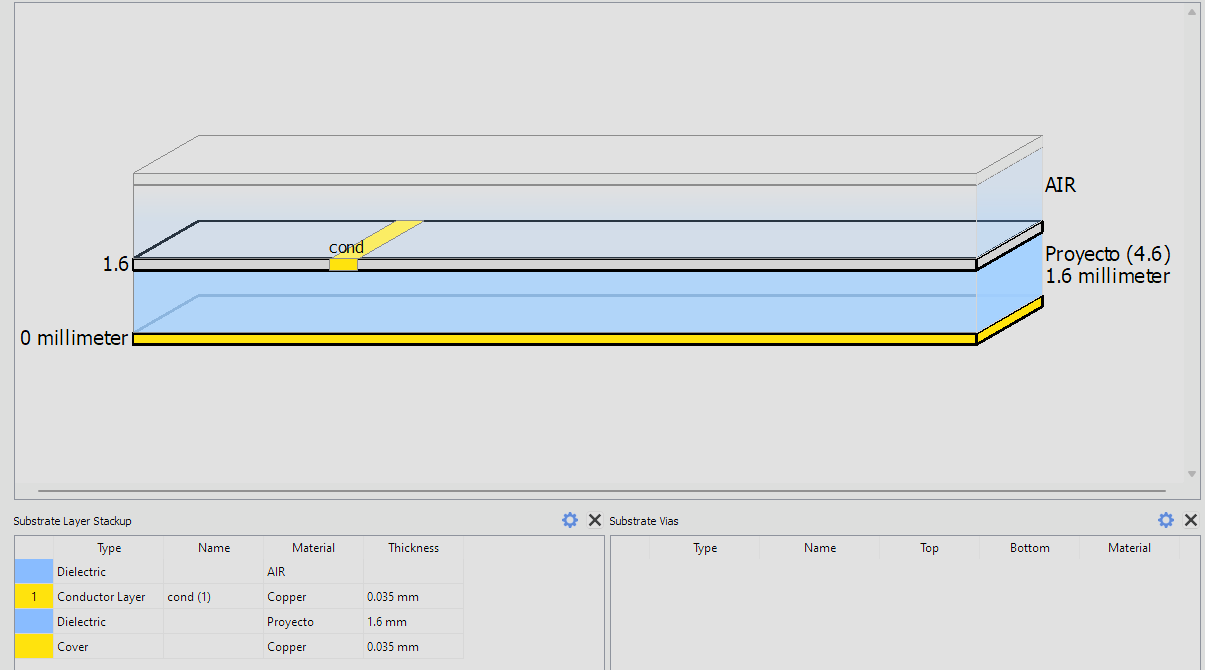
\includegraphics[width=8cm]{figures/metodologia/metologia4.png}
    \caption{Capas del substrato}
    \label{fig:metologia_substrato}
\end{figure}

\subsection{Simulación electromágnetica}

Haga click derecho sobre la carpeta que contiene el layout y seleccione la opción \texttt{New} y posteriormente \texttt{EmSetup}. Seleccione con doble click el archivo creado.
En la pestaña de \texttt{Ports} refresce la información utilizando las 2 flechas verdes en la parte superior izquierda de la ventana. Posteriormente, regrese a la pestaña \texttt{FEM} y seleccione el tipo de simulación \texttt{EM Simulation/Model} utilizando el simulador \texttt{FEM}. En la parte inferior derecha selecciona la opción para generar parámetros y precione el botón \texttt{Simulate}.
